\chapter{ブラックホールエントロピー、ホログラフィー、ド・ジッター空間}

\lectureoverview{前回の講義で始めた対応関係の議論を完成させる。強く励起された弦のエントロピーはその質量に比例し、シュヴァルツシルトブラックホールのエントロピーはその面積に比例する。二つの式は、強い重力を持つブラックホールを自由な弦と同一視することによってではなく、二つの記述が出会うまで弦結合定数をゆっくり変化させることによって結びつけられる。面積則はそこから自然にホログラフィー原理へと導き、講義の最後の部分では膨張する空間と、次にその地平線を調べることになるド・ジッター幾何学を導入する。}

\section{数え上げの問題に戻る}

長い弦の数え上げには未解決の点が一つあった。固定された全長がいくつかの弦に分割される場合、同じ長さの同一の弦は区別できない。それでも箱の中のそれらの位置は状態の一部であり、箱は対応する単一の長い弦が占めるのとほぼ同じ大きさに選ばれる。

\begin{classroomqa}
\audiencequestion{短い弦は互いに区別されるのか、またそれらの位置は数えられるのか。\lecturetimestamp{00:00:37}}
\lecturerresponse{同一の性質を持つ弦は区別できないが、箱の中のそれらの位置は数えられる。比較は固定された体積で行われ、長い弦が占める領域に合わせて選ばれる。}
\end{classroomqa}

それが片づいたので、目標を述べることができる。短い式のリストをまとめ、それらを用いてブラックホールエントロピーのスケーリングを導く。積分も無限和も必要ない。困難は代数的なものではなく、どの量をどの段階で比較してよいかを知ることにある。

\section{自然単位とプランク面積}

次のように置く。
\begin{equation}
c=\hbar=1,
\label{eq:l07-natural-units}
\end{equation}
ただしニュートン定数はあらわに残す。最初の帰結は、時間と長さが同じ単位を持つことである。光子の関係式
\begin{equation}
E=\frac{\hbar c}{\lambda}
\end{equation}
と質量とエネルギーの関係式\(E=mc^2\)から
\begin{equation}
[M]=L^{-1}.
\label{eq:l07-mass-dimension}
\end{equation}
が従う。したがって質量は逆長さとして表すことができる。

\begin{figure}[htbp]
\centering
\includegraphics[width=0.62\textwidth]{lecture_07_figure_02.png}
\caption{次元解析の冒頭における自然単位の規約。エネルギー公式は上の式で完成する。}
\lectureframe{00:03:27.900}
\end{figure}

\(G_N\)の単位を決めるには、ニュートン加速度を次元の帳尻合わせとしてのみ用いる。
\begin{equation}
a\sim\frac{G_NM}{R^2}.
\end{equation}
\(T\)と\(L\)は同じ単位を持つので、\([a]=L/T^2=L^{-1}\)である。式~\eqref{eq:l07-mass-dimension}と合わせて
\begin{equation}
[G_N]=L^2.
\end{equation}
が得られる。ニュートン定数はこれらの単位では面積である。プランク長を
\begin{equation}
G_N=\ell_p^2,
\label{eq:l07-planck-area}
\end{equation}
で定義すれば、\(A/G_N=A/\ell_p^2\)が無次元である理由は直ちに理解できる。すなわちプランク面積の単位で面積を測っているのである。

\section{弦結合定数と重力の強さ}

重力を今度は弦の言葉に翻訳しなければならない。有用な描像は交換過程である。弦が自分自身と交差すると、分裂して再結合することがある。小さな閉弦ループが一方の物体から放出され他方に吸収されることがあり、その励起が重力子であるとき、この過程が重力を媒介する。放出で一つの相互作用因子が現れ、吸収でもう一つ現れるので、交換の強さには\(g_s^2\)が含まれる。

結合定数\(g_s\)は無次元である。より正確には、それは振幅レベルの結合定数であり、確率や率は\(g_s^2\)の次数から始まる。\editorialnote{講義では時に\(g_s\)を確率と呼び、それを確率の平方根と訂正する。摂動的な結合定数は振幅レベルに属する。} \(G_N\)は面積の次元を持つので、依然として長さのスケールが欠けている。基本弦の長さ\(\ell_s\)、すなわち一つの素的な弦の揺れのスケールがそれを与える。
\begin{equation}
G_N\sim g_s^2\ell_s^2,
\qquad
\ell_p\sim g_s\ell_s.
\label{eq:l07-planck-string}
\end{equation}

\begin{figure}[htbp]
\centering
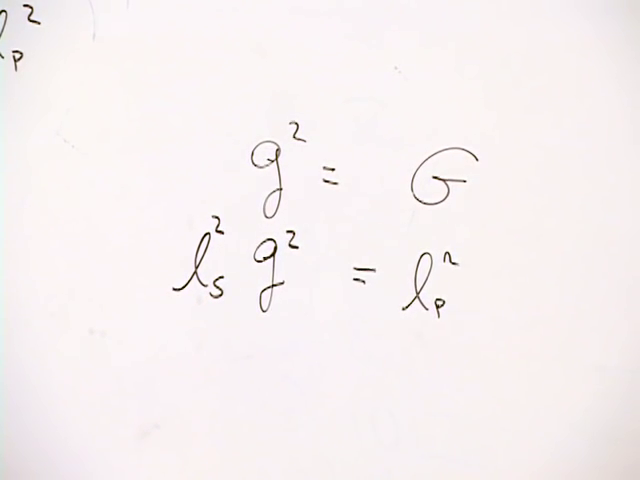
\includegraphics[width=0.72\textwidth]{lecture_07_figure_05.png}
\caption{黒板に書かれた結合定数の関係: \(G_N=\ell_p^2\)および\(g_s^2\ell_s^2\sim\ell_p^2\)。}
\lectureframe{00:12:15.000}
\end{figure}

弱結合\(g_s\ll1\)では、プランク長は弦の長さよりずっと小さい。\(g_s\)を小さくすると、素的な弦のスケールを固定したまま重力が弱くなる。\editorialnote{有効四次元理論では、コンパクト化のデータと数値的な規約も\(G_N\)に入ってくる。それらはこのスケーリングの議論では固定され、抑えられている。}

\section{長い弦の数え上げ}

エントロピーは、状態を指定するのに必要な素的な決定の数を数える。強く励起された弦を正方形格子上の歩みに置き換える。各頂点で次の辺は四つの方向のいずれかを向きうる。素的な選択を一つの四択の決定として記述するか二つの二択の決定として記述するかは、一次の定数を変えるだけである。重要なのは歩数の数である。

\(L\) が弦の輪郭長であり、各ステップの長さが \(\ell_s\) であるならば、
\begin{equation}
N=\frac{L}{\ell_s}
\end{equation}
ステップが必要である。ウォークの数は指数的に増大し、模式的には \(\Omega_N\sim q^N\) で、\(q\) は1の程度であり、したがって
\begin{equation}
S_{\mathrm{str}}=\log\Omega_N\sim N\sim\frac{L}{\ell_s}.
\label{eq:l07-string-entropy-length}
\end{equation}

\begin{figure}[htbp]
\centering
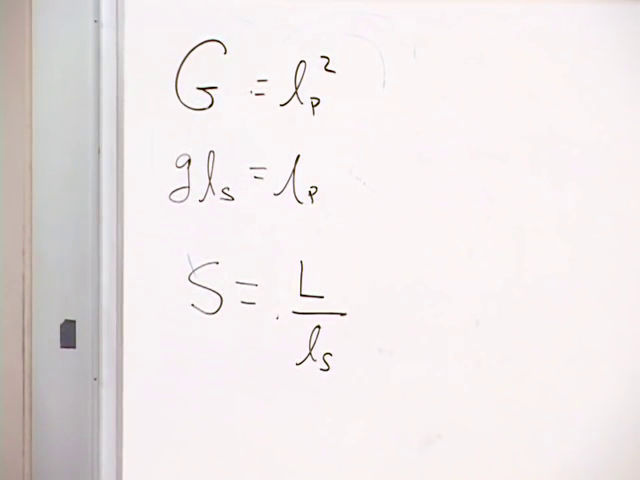
\includegraphics[width=0.68\textwidth]{lecture_07_figure_03.png}

\vspace{0.7em}
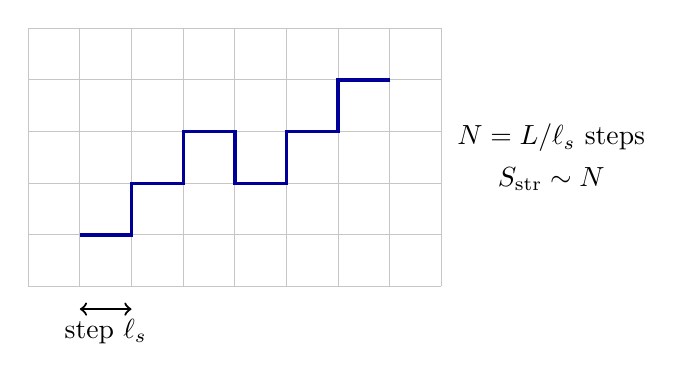
\begin{tikzpicture}[scale=0.82]
  \draw[step=0.8cm,gray!45,thin] (0,0) grid (6.4,4.0);
  \draw[very thick,blue!60!black]
    (0.8,0.8)--(1.6,0.8)--(1.6,1.6)--(2.4,1.6)--(2.4,2.4)--
    (3.2,2.4)--(3.2,1.6)--(4.0,1.6)--(4.0,2.4)--(4.8,2.4)--
    (4.8,3.2)--(5.6,3.2);
  \draw[<->,thick] (0.8,-0.35)--(1.6,-0.35);
  \node[below] at (1.2,-0.35) {step \(\ell_s\)};
  \node[align=center] at (8.1,2.0) {\(N=L/\ell_s\) steps\\[0.3em]\(S_{\mathrm{str}}\sim N\)};
\end{tikzpicture}
\caption{黒板上の格子模型とその整理されたランダムウォーク解釈。選択肢の数を決めるのは、もつれた球の直径ではなく輪郭長である。}
\lectureframe{00:17:20.000}
\end{figure}

質量は同じ基本セグメントから数えられる。長さ \(\ell_s\) のセグメントは質量スケール
\begin{equation}
m_{\mathrm{seg}}\sim\frac{1}{\ell_s}.
\end{equation} をもつ

\begin{classroomqa}
\audiencequestion{基本セグメントに長さ \(\ell_s\) が割り当てられているのか。\lecturetimestamp{00:18:56}}
\lecturerresponse{はい。その特徴的長さは \(\ell_s\) であるので、自然単位ではその特徴的質量は \(1/\ell_s\) である。}
\end{classroomqa}

\(L/\ell_s\) 個のセグメント質量を加えると
\begin{equation}
M\sim\frac{L}{\ell_s}\frac{1}{\ell_s}
=\frac{L}{\ell_s^2},
\qquad
L\sim M\ell_s^2.
\label{eq:l07-string-mass}
\end{equation}
振動する弦の運動エネルギーとポテンシャルエネルギーはこのスケーリング関係に圧縮されている。詳細な統計力学的取り扱いでも同じ依存性が得られる。式~\eqref{eq:l07-string-entropy-length}に代入すると、我々が必要とする弦の公式が得られる：
\begin{equation}
S_{\mathrm{str}}\sim M\ell_s.
\label{eq:l07-string-entropy-mass}
\end{equation}

\begin{figure}[htbp]
\centering
\includegraphics[width=0.66\textwidth]{lecture_07_figure_04.png}
\caption{比較の前にまとめられた弦側の列：\(\ell_p\sim g_s\ell_s\)、\(S_{\mathrm{str}}\sim L/\ell_s\sim M\ell_s\)、および \(M\sim L/\ell_s^2\)。}
\lectureframe{00:21:57.800}
\end{figure}

\section{なぜ自由弦はまだブラックホールではないのか}

重力側では、厳密な半古典的公式は
\begin{equation}
S_{\mathrm{BH}}=\frac{A}{4G_N}.
\label{eq:l07-bh-exact}
\end{equation} である

\begin{classroomqa}
\audiencequestion{分母に入る数値係数は何か。\lecturetimestamp{00:23:28}}
\lecturerresponse{4。対応関係の議論はスケーリングを再現するが、その厳密な因子を決定するには粗すぎる。}
\end{classroomqa}

4次元シュヴァルツシルトブラックホールに対して、
\begin{equation}
R_s=2G_NM,
\qquad
A=4\pi R_s^2.
\end{equation}
講義で行ったように数値定数を落とすと、
\begin{align}
S_{\mathrm{BH}}
&\sim\frac{A}{G_N}
\sim\frac{(G_NM)^2}{G_N} \\
&\sim M^2G_N
\sim M^2\ell_p^2.
\label{eq:l07-bh-scaling}
\end{align}

\begin{figure}[htbp]
\centering
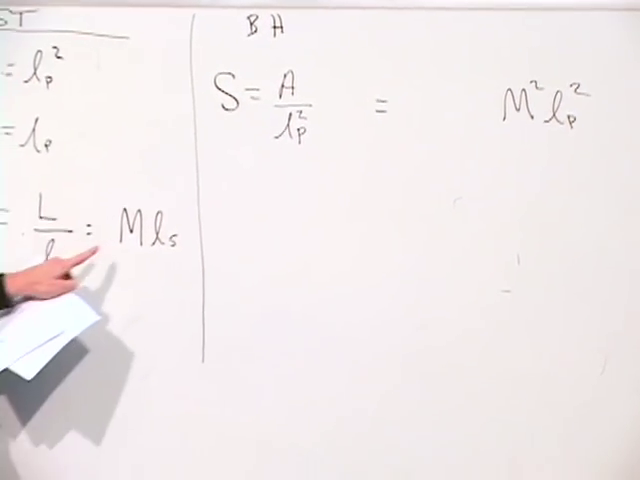
\includegraphics[width=0.72\textwidth]{lecture_07_figure_06.png}
\caption{黒板上で完成した比較：弦のエントロピーは弦単位での長さであるのに対し、ブラックホールのエントロピーはプランク単位での面積である。}
\lectureframe{00:25:35.000}
\end{figure}

式~\eqref{eq:l07-string-entropy-mass}と式\eqref{eq:l07-bh-scaling}の類似は示唆的であるが、それらは同じ公式ではない。元のブラックホールを単に自由弦と呼んで代入するのは誤りであろう。自由弦の数え上げは弦の部分間の引力相互作用を省略しており、まさにその相互作用が弦をブラックホールへと圧縮し、負の結合エネルギーを通じてその全エネルギーを下げるのである。

恒星はこの誤りを身近なものにする。恒星質量の高温ガスを大きすぎる箱に入れたものは、同じ温度であっても恒星の模型ではない。自己重力が平衡サイズとエネルギー・エントロピー関係を変える。長い弦のあらゆる自己相互作用を追跡するのは困難であろうから、我々はそうすることを避ける。

\begin{classroomqa}
\audiencequestion{小さなループが長い弦から離れると、そのエントロピーは減少する。では重力子の交換は重力系のエントロピーを下げるのか。\lecturetimestamp{00:28:48}}
\lecturerresponse{ここで用いている平衡交換過程ではそうではない。仮想励起は両方向に放出・吸収される。この絵は永続的な弦の断片の文字通りの損失ではない。その現在の唯一の目的は、2つの結合因子、したがって \(g_s^2\) 依存性を確立することである。}
\end{classroomqa}

\section{断熱対応ゲーム}

代わりに重力が無視できるところから始めよう。\(g_s\to0\) では、弦は分裂も結合もせずに交差し、自己重力引力は消える。\(\ell_s\) を固定したまま \(g_s\) を増加させる：重力が強まり、高度に励起された弦は収縮し、最終的にブラックホールになる。ダイヤルをゆっくり逆に回すと、ブラックホールは弦状態に戻らなければならない。それは少数の長い弦になるかもしれないが、前回の講義の高エネルギー数え上げによれば、支配的なセクターは短い弦の巨大なガスではなく1本の長い弦を含む。

\begin{classroomqa}
\audiencequestion{結合が変化する間、何が固定されているのか。\lecturetimestamp{00:32:19}}
\lecturerresponse{弦の長さ \(\ell_s\)、したがって基本弦質量スケール \(1/\ell_s\) が固定されている。ダイヤルは \(g_s\) を変え、それゆえ \(G_N\sim g_s^2\ell_s^2\) を変える。}
\end{classroomqa}

変化は遅く、孤立しており、可逆でなければならない。そのような条件下でエントロピーは断熱不変量である：
\begin{equation}
\Delta S=0.
\label{eq:l07-adiabatic}
\end{equation}
散逸的または制御されていない遷移が起こるならば、遅いだけでは十分ではない。ここで ``断熱'' とは、同じ状態の族を連続的に追跡できることを意味する。\editorialnote{これは断熱の可逆熱力学的な意味である。不可逆過程は熱流なしの意味で断熱的でありながら、なおエントロピーを生成しうる。}

対象とするブラックホールの質量を\(M_0\)、結合を\(g_{s,0}\)とする。これから説明しようとしている面積公式を使う前に、次元解析が言えるのは、中性で回転していないブラックホールのエントロピーは無次元の組み合わせ
\begin{equation}
S_{\mathrm{BH}}=f(M\ell_p)
=f(Mg_s\ell_s).
\label{eq:l07-entropy-function}
\end{equation}
のある関数であるということだけである。\(\ell_s\)を固定すると、等エントロピー経路はしたがって
\begin{equation}
Mg_s=M_0g_{s,0}
\label{eq:l07-adiabat}
\end{equation}
を一定に保つ。ただし、同じ状態の枝に沿って進む場合に限る。

\(g_s\)が減少するにつれて、負の結合エネルギーが取り除かれるので、この経路に沿って質量\(M\)は増大する。背後にある弦の配位もより強く束縛されなくなり、広がっていく。しかし、形式的なシュヴァルツシルト半径は断熱経路上で\(R_s\sim Mg_s^2\ell_s^2\sim g_s\ell_s\)のように振る舞うため、減少する。\editorialnote{口頭の議論では、重力結合から解放された物体について``grows''という表現が使われている。これは、導出された断熱経路に沿ってシュヴァルツシルト半径が増大するという意味に読んではならない。}

\begin{classroomqa}
\audiencequestion{重力が弱められると、この物体は成長するのか、それとも縮むのか。\lecturetimestamp{00:36:28}}
\lecturerresponse{その弦構造は解放されて膨張する一方、負の結合エネルギーが取り除かれるため質量は増大する。ブラックホールの公式が割り当てる半径は、弦のスケールに達するまで減少し、そこではそのブラックホール的記述はもはや有用でなくなる。}
\end{classroomqa}

\section{二つの曲線とその交点}

質量を縦軸に、弦結合を横軸にとる。式~\eqref{eq:l07-adiabat}は双曲線であり、\(M\propto g_s^{-1}\)である。

\begin{classroomqa}
\audiencequestion{積\(Mg_s\)が一定であるような曲線は何か。\lecturetimestamp{00:44:08}}
\lecturerresponse{双曲線である。それは目標点\((g_{s,0},M_0)\)を通る断熱経路である。}
\end{classroomqa}

第二の曲線は、二つの記述の間のクロスオーバーを表す。ブラックホールは、その半径が素弦の揺らぎより小さくなると、通常のシュヴァルツシルト幾何として解像できなくなる。したがって、対応点を
\begin{equation}
R_s\sim\ell_s.
\label{eq:l07-correspondence-radius}
\end{equation}
によって見積もる。\(R_s\sim MG_N\)と式~\eqref{eq:l07-planck-string}を用いると、これは
\begin{equation}
Mg_s^2\ell_s^2\sim\ell_s,
\qquad
Mg_s^2\sim\frac{1}{\ell_s}.
\label{eq:l07-transition-curve}
\end{equation}
となる。したがって、転移曲線は\(M\propto g_s^{-2}\)として減少し、断熱経路よりも急である。

\begin{figure}[htbp]
\centering
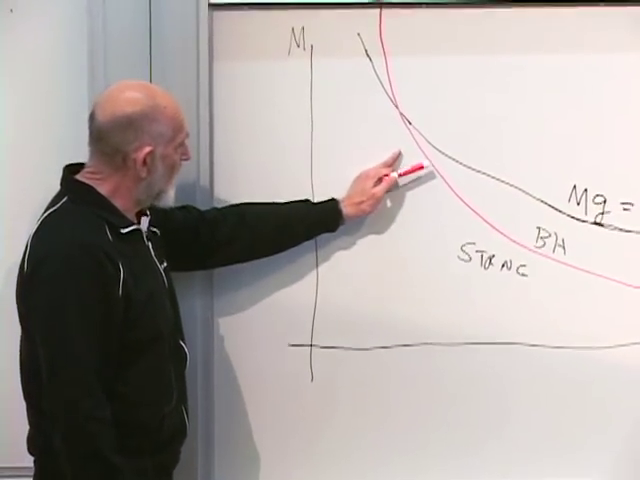
\includegraphics[width=0.70\textwidth]{lecture_07_figure_07.png}

\vspace{0.6em}
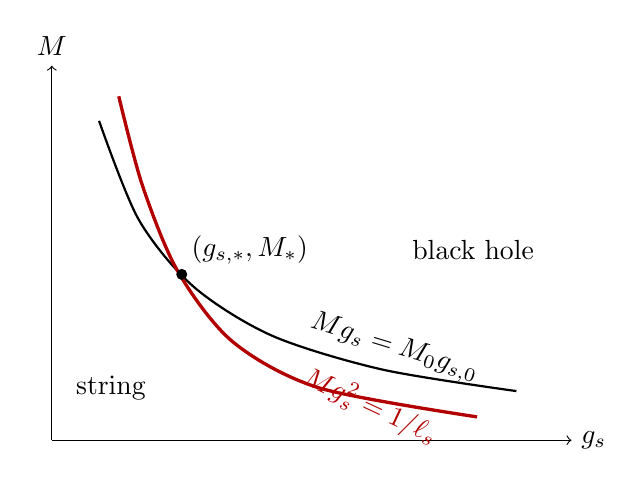
\begin{tikzpicture}[x=1cm,y=0.78cm]
  \draw[->] (0.4,0.4)--(7.0,0.4) node[right] {\(g_s\)};
  \draw[->] (0.4,0.4)--(0.4,6.5) node[above] {\(M\)};
  \draw[thick,black] plot[smooth] coordinates {(1.0,5.6) (1.5,4.0) (2.2,2.9) (3.2,2.1) (4.6,1.55) (6.3,1.2)};
  \draw[very thick,red!70!black] plot[smooth] coordinates {(1.25,6.0) (1.55,4.55) (2.0,3.15) (2.7,2.0) (3.8,1.25) (5.8,0.78)};
  \fill (2.05,3.1) circle (2pt) node[above right] {\((g_{s,*},M_*)\)};
  \node[black,rotate=-17] at (4.75,1.9) {\(Mg_s=M_0g_{s,0}\)};
  \node[red!70!black,rotate=-25] at (4.45,0.95) {\(Mg_s^2=1/\ell_s\)};
  \node at (5.75,3.5) {black hole};
  \node at (1.15,1.25) {string};
\end{tikzpicture}
\caption{黒板のグラフとその整理された解釈。黒い断熱経路は、物体が弦的になる点で、より急な赤い対応曲線と交わる。}
\lectureframe{00:49:35.000}
\end{figure}

交点\((M_*,g_{s,*})\)において、二つの方程式は
\begin{align}
M_*g_{s,*} &= M_0g_{s,0}, \\
M_*g_{s,*}^2 &\sim \frac{1}{\ell_s}.
\end{align}
である。第一の式を二乗し、第二の式で割ると、
\begin{equation}
M_*
\sim M_0^2g_{s,0}^2\ell_s.
\end{equation}
となる。\(\ell_s\)を掛けると、
\begin{equation}
M_*\ell_s
\sim M_0^2g_{s,0}^2\ell_s^2
\sim M_0^2G_{N,0}.
\label{eq:l07-crossover-result}
\end{equation}

\begin{figure}[htbp]
\centering
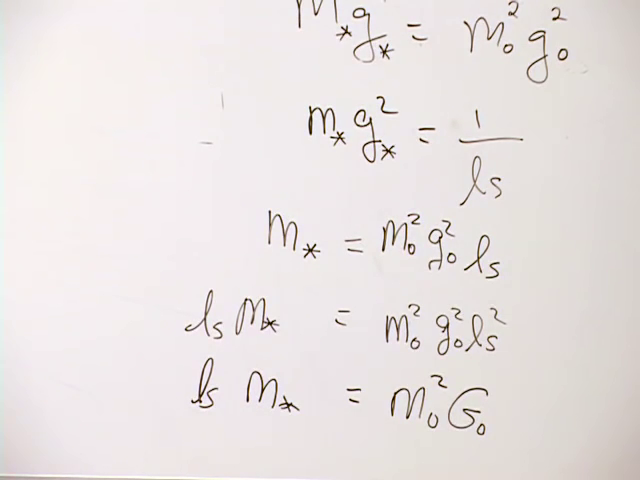
\includegraphics[width=0.68\textwidth]{lecture_07_figure_08.png}
\caption{\(M_*\ell_s=M_0^2g_{s,0}^2\ell_s^2=M_0^2G_{N,0}\)を含む、完成したクロスオーバー代数。}
\lectureframe{00:54:40.000}
\end{figure}

\begin{classroomqa}
\audiencequestion{二つの曲線の方程式を割ると、\(\ell_s\)は分子に来るべきか、それとも分母に来るべきか。\lecturetimestamp{00:52:41}}
\lecturerresponse{分子に来る。\(1/\ell_s\)で割ることは\(\ell_s\)を掛けることであり、そのため\(M_*\sim M_0^2g_{s,0}^2\ell_s\)となる。}
\end{classroomqa}

クロスオーバーでは弦の公式が有効なので、
\begin{equation}
S_*\sim M_*\ell_s.
\end{equation}
である。経路に沿ってエントロピーは変化しなかった。この主張を式~\eqref{eq:l07-crossover-result}と組み合わせると、元の対象ブラックホールのエントロピーが得られる：
\begin{equation}
S_{\mathrm{BH}}(M_0)
\sim M_0^2G_{N,0}
\sim M_0^2\ell_{p,0}^2.
\label{eq:l07-final-correspondence}
\end{equation}
これが求める面積則のスケーリングである。

\section{対応関係が証明することと証明しないこと}

この構成は、元の強い重力を持つブラックホールが自由な弦であるとは述べていない。物体を弦の数え上げが信頼できる領域へ移し、そこでエントロピーを読み取り、そのエントロピーを可逆な経路に沿って元へ運び戻すのである。転移は鋭く位置づけられた相境界ではなくクロスオーバーであるため、この見積もりでは式~\eqref{eq:l07-bh-exact}の係数\(1/4\)を決定することはできない。

それでも同じ論理は、荷電ブラックホール、他の次元のブラック物体、および拡張されたブラックブレーンに対してパラメトリックに機能する。より対称性が高く超対称な例では、結合が変化しても厳密な情報を保つ保護された状態の数え上げが可能である。それらの方法は数値係数を回復するが、現在の概念的議論には不要な数学的装置を追加する。

最も重要なのは、この計算が微視的解釈を与えることである。エントロピーは隠れた構造の証拠である。流体力学は分子を省いて密度、圧力、流れを記述するが、流体のエントロピーはそのような微視的自由度が存在することを明らかにする。一般相対性理論も同様に、その微視的状態を明示することなく事象の地平面を記述する。弦の数え上げは、重力の整合的な量子論がブラックホールのエントロピーを説明するのに十分な状態を含みうることを示している。

\begin{classroomqa}
\audiencequestion{二次の結果の代わりに\(S\sim M^3\ell_p^3\)だったなら、何を意味しただろうか。\lecturetimestamp{00:59:41}}
\lecturerresponse{それは体積則のように見えたであろう。部屋の中の普通の物質や一杯のコーヒーは体積に比例するエントロピーを持つ。二次の答えが特別なのは、\(R_s\sim M\ell_p^2\)を通じて、それが地平面の面積に比例するからである。}
\end{classroomqa}

この結果は、ベッケンシュタイン--ホーキングエントロピーが単なる形式的な熱力学的類推ではないことの証拠である。それは微視的な重力自由度を示唆している。ただし、初等的な導出はそれらの自由度を一つ一つ可視化するものではない。

\section{最大エントロピーからホログラフィーへ}

ここで問いを変える。指定された状態のエントロピーを問う代わりに、ある領域と両立する最大のエントロピーを問う。

部屋の通常の格子模型から始める。体積を大きさ\(V_{\mathrm{cell}}\)のセルに分割し、各セルに一つのイエス・ノーの問いを持たせる。すなわち占有か空かである。ススキンドは想像上の原子に、意図的にばかげた名前``meatonium''を与える。現実的な原子の詳細が数え上げの妨げにならないようにするためである。もし
\begin{equation}
N=\frac{V}{V_{\mathrm{cell}}},
\end{equation}
ならば、配位の数と最大エントロピーは
\begin{equation}
\Omega=2^N,
\qquad
S_{\max}=\log\Omega=N\log2
\sim\frac{V}{V_{\mathrm{cell}}}.
\label{eq:l07-volume-count}
\end{equation}

\begin{figure}[htbp]
\centering
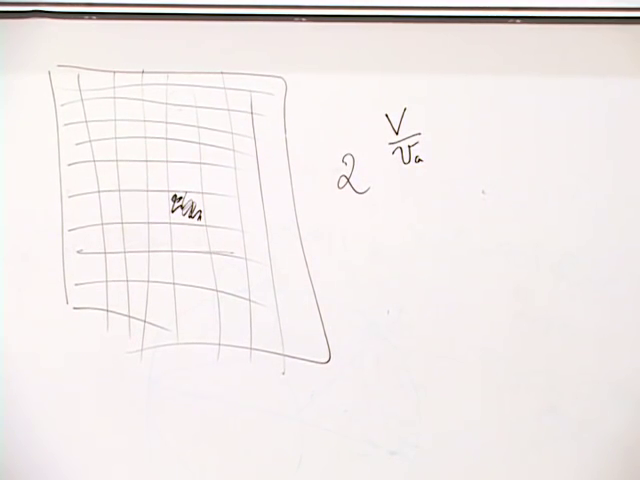
\includegraphics[width=0.68\textwidth]{lecture_07_figure_09.png}
\caption{セルに分割された部屋。各セルは二つの状態を持つ。これは最大エントロピーを数えており、授業が占める整然とした部屋のエントロピーではない。}
\lectureframe{01:05:20.000}
\end{figure}

実際の部屋はこの最大値よりはるかに低い。それらすべてのセルの選択を混沌と探索する状態は極めて高温であろう。おもちゃの模型から生き残るのは、独立な自由度の数、したがって最大エントロピーが体積に比例するという通常の期待である。

重力はその期待を覆す。境界面積\(A\)、初期エントロピー\(S_{\mathrm{i}}\)、質量\(M\)を持ち、その球をちょうど満たすブラックホールの質量\(M_{\mathrm{BH}}\)より小さい球状領域を考える。もし\(M\)がより大きければ、その事象の地平面はすでに選んだ境界を越えて広がっているであろう。

次に質量\(M_{\mathrm{BH}}-M\)の殻を送り込む。その組成は無関係である。講義は光、通常の物質、あるいはスイスチーズさえも許容する。それが崩壊するように整える。最終状態は、地平面がちょうどその領域を満たすブラックホールであり、エントロピーは
\begin{equation}
S_{\mathrm{f}}=\frac{A}{4G_N}.
\end{equation}
第二法則は次を要求する
\begin{equation}
S_{\mathrm{i}}\le S_{\mathrm{f}}
=\frac{A}{4G_N}.
\label{eq:l07-holographic-bound}
\end{equation}

\begin{figure}[htbp]
\centering
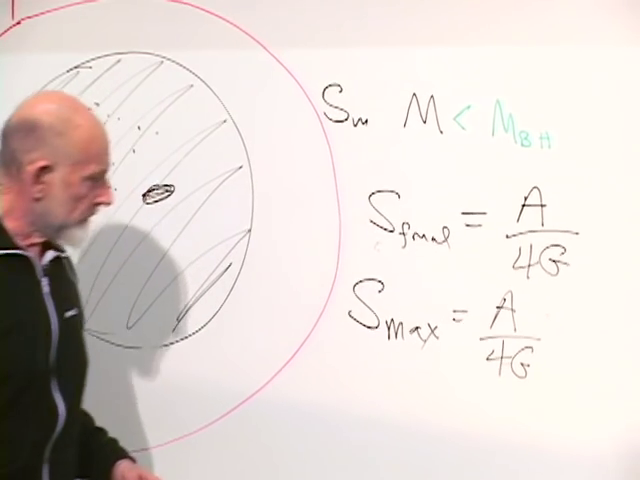
\includegraphics[width=0.70\textwidth]{lecture_07_figure_10.png}

\vspace{0.5em}
\begin{tikzpicture}[scale=0.88]
  \draw[thick] (0,0) circle (1.35);
  \draw[very thick,red!70!black] (0,0) circle (2.05);
  \fill[gray!25] (0,0) circle (1.32);
  \node at (0,0) {\(M,S_{\mathrm{i}}\)};
  \draw[-{Latex[length=3mm]},thick,red!70!black] (3.5,0)--(2.15,0);
  \node[align=center,right] at (3.5,0) {incoming shell\\\(M_{\mathrm{BH}}-M\)};
  \node[below] at (0,-2.2) {final horizon area \(A\)};
\end{tikzpicture}
\caption{殻の構成。選ばれた領域をちょうど満たす地平面を持つブラックホールを形成するのに十分な追加質量が内側へ送り込まれる。}
\lectureframe{01:13:30.000}
\end{figure}

その大きさのブラックホールは許される状態であり、不等式を飽和させるので、最大エントロピーは
\begin{equation}
S_{\max}=\frac{A}{4G_N}.
\label{eq:l07-holographic-maximum}
\end{equation}
これが数え上げの形でのホログラフィー原理である。重力のある領域における独立な自由度の最大数は、内部のプランク体積の数ではなく、その境界の面積に比例し、およそプランク面積あたり1桁程度の自由度である。\editorialnote{殻の議論は、その領域が述べられた方法で囲まれ崩壊できることを仮定している。より一般的な時空には共変的エントロピー境界が必要であるが、球対称の議論は講義で用いられた原理を捉えている。}

その隔たりは莫大である。局所場の理論の直観は、異なる内部点でなされた選択が独立に結合し、体積則を生み出すことを示唆する。重力は、そのような選択が十分に多ければそれ自体が崩壊し、ブラックホールがより大きな許容エントロピーを与えると言う。したがって境界の数え上げは体積の数え上げに対する小さな補正ではなく、ヒルベルト空間の異なる組織化である。

\begin{classroomqa}
\audiencequestion{ほぼ一様な密度を持つ非常に大きな宇宙では何が起こるか。\lecturetimestamp{01:15:48}}
\lecturerresponse{その問いは静的で球対称な構成ではなく宇宙論を必要とする。それはアインシュタイン方程式の膨張解への即座の移行を動機づける。}
\end{classroomqa}

\begin{classroomqa}
\audiencequestion{面積の境界は不確定性原理と関係しているか。\lecturetimestamp{01:16:03}}
\lecturerresponse{講義はこの問いを未解決のまま残し、次に宇宙論へ移る。}
\end{classroomqa}

\section{膨張する空間}

ここではアインシュタイン方程式から宇宙論的解を導出しない。解を書き下し、その読み方を学ぶ。空間的スライスは正に曲がって閉じているか、負に曲がって双曲的であるか、平坦でありうる。当面の議論では、時間依存の時空における空間的に平坦なユークリッド的スライスを取る。

\begin{classroomqa}
\audiencequestion{通常のユークリッド空間の時空版は何か。\lecturetimestamp{01:19:37}}
\lecturerresponse{ミンコフスキー空間である。ここで考える宇宙論は平坦な空間的スライスを持つが、その空間計量が時間とともに変化するため、ミンコフスキー時空ではない。}
\end{classroomqa}

おなじみの風船の描像は、1次元低い閉じた膨張面を表している。Susskindは、大きな印を付けた風船で実演を試みたことを回想している。マーカーがゴムを弱め、文字通りパンという音が生じた。この失敗は、この類推における概念的欠陥も露呈させる。普通の風船が膨張すると、そのゴム分子は離れていき、材料は薄くなってついには破れる。宇宙論的な空間は、薄められた局所的法則を獲得するわけではない。類推を保つには、新たなゴム分子を絶えず挿入し、あらゆる小さなパッチが同じ局所的性質を保つように想像しなければならない。平坦な模型では、風船を、一様に外側へ引っ張られ同様に補充される大きなシートに置き換える。

数学的には、膨張は計量に属する：
\begin{equation}
\begin{aligned}
ds^2&=-dt^2+a(t)^2d\mathbf{x}^2,\\
d\mathbf{x}^2&=\delta_{ij}\,dx^i dx^j
=dx^2+dy^2+dz^2.
\end{aligned}
\label{eq:l07-frw-metric}
\end{equation}

\begin{figure}[htbp]
\centering
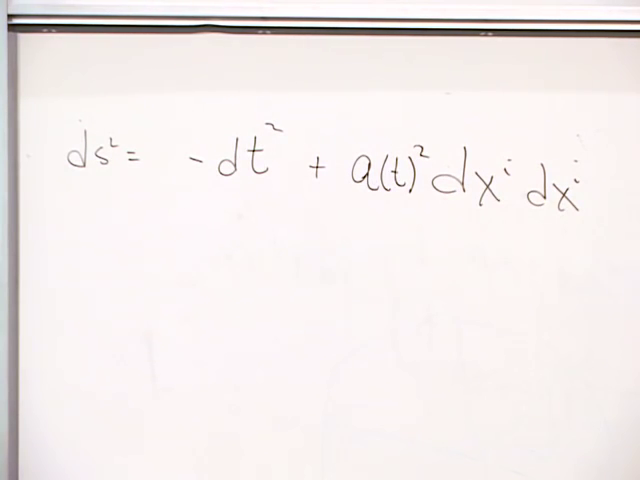
\includegraphics[width=0.72\textwidth]{lecture_07_figure_11.png}
\caption{黒板に書かれた、そのままの空間的に平坦な膨張計量。}
\lectureframe{01:25:10.000}
\end{figure}

固定された空間座標を保つ点は共動と呼ばれる。そのような2点が座標間隔\(\Delta x\)を持つとき、時刻\(t\)におけるそれらの固有距離は
\begin{equation}
D(t)=a(t)\Delta x.
\label{eq:l07-proper-distance}
\end{equation}
である。それらの座標は動かないが、それらの間の計量的距離は変化する。\(\Delta x\)を固定して微分すると、
\begin{equation}
V=\dot D=\dot a\,\Delta x
=\frac{\dot a}{a}D.
\end{equation}
ハッブルパラメータを
\begin{equation}
H(t)=\frac{\dot a(t)}{a(t)}.
\label{eq:l07-hubble-parameter}
\end{equation}
と定義する。すると
\begin{equation}
V=H(t)D,
\label{eq:l07-hubble-law}
\end{equation}
となり、これは固定された宇宙時刻におけるハッブルの法則である。

\begin{figure}[htbp]
\centering
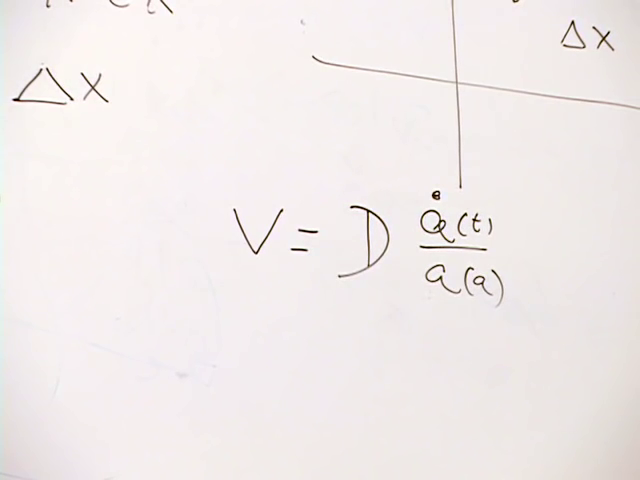
\includegraphics[width=0.68\textwidth]{lecture_07_figure_12.png}
\caption{黒板に書かれた等時後退法則：\(V=D\,\dot a/a\)。}
\lectureframe{01:29:10.000}
\end{figure}

``ハッブル定数''という名称は誤解を招きうる。一般に\(H(t)\)は時間とともに変化する。空間的に一定なのは、同じ時間スライス上のあらゆる共動点の対に対する比\(V/D\)である。

\begin{classroomqa}
\audiencequestion{遠方の銀河について、この関係に現れる時刻は誰の時刻か。我々はそれらをより早い時代に観測する。\lecturetimestamp{01:31:10}}
\lecturerresponse{式~\eqref{eq:l07-hubble-law}は等時的な主張である。観測は過去向きの光線に沿って進み、遠方の銀河をより早い時刻にサンプルする。したがって、測定された赤方偏移と距離の関係には、\(H\)の一瞬の値ではなく、光円錐の全履歴が必要である。}
\end{classroomqa}

\begin{figure}[htbp]
\centering
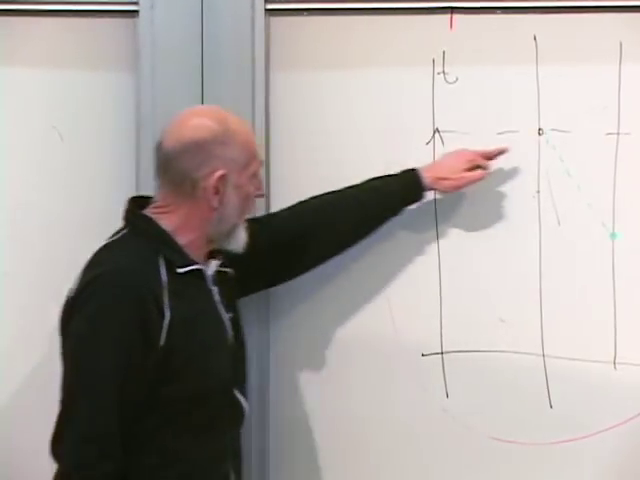
\includegraphics[width=0.66\textwidth]{lecture_07_figure_13.png}
\caption{等時的分離と、観測者が過去の光線に沿って見るものとを区別するために用いられる時空のスケッチ。}
\lectureframe{01:33:20.000}
\end{figure}

\section{ハッブルスケールとド・ジッター膨張}

単位\(c=1\)では、式~\eqref{eq:l07-hubble-law}は距離
\begin{equation}
D_H=\frac{1}{H}.
\label{eq:l07-hubble-radius}
\end{equation}
において後退速度を1に定める。より遠方の共動点は、特殊相対性理論に違反することなく\(V>1\)、あるいは\(V\gg1\)さえ持ちうる。それらは局所的な観測者を光より速く通過するのではない。それらの固有分離は、間にある幾何が膨張するために増大する。\editorialnote{一般の時間依存の宇宙論では、\(1/H\)はハッブル半径であり、自動的に事象の地平面になるわけではない。次に議論するド・ジッターの場合には、それが一定の地平面スケールとなる。}

多くの古い減速する宇宙論的模型では、\(H(t)\)は減少し\(1/H(t)\)は増大するので、かつて超光速で後退していた領域が後に因果的接触に入りうる。講義で議論される晩期の描像は、代わりに正の定数\(H\)に近づく。すると\(1/H\)は固定されたままであり、膨張方程式は
\begin{equation}
\frac{\dot a}{a}=H,
\qquad
\dot a=Ha.
\label{eq:l07-constant-h}
\end{equation}
となる。

\begin{classroomqa}
\audiencequestion{一定のハッブルパラメータの単位は何か。\lecturetimestamp{01:38:24}}
\lecturerresponse{時間の逆数である。等価に、\(c=1\)とすれば、長さの逆数である。量\(H^{-1}\)は膨張時間と距離スケールの両方を与える。講義では約150億年という桁の例を用いている。}
\end{classroomqa}

式~\eqref{eq:l07-constant-h}の解は
\begin{equation}
a(t)=a_0e^{Ht}.
\label{eq:l07-desitter-scale-factor}
\end{equation}
である。

\begin{classroomqa}
\audiencequestion{それ自身に比例する変化率を持つ関数は何か。\lecturetimestamp{01:39:04}}
\lecturerresponse{指数関数である。したがってスケール因子は\(a_0e^{Ht}\)であり、一方、計量における空間係数\(a(t)^2\)は\(e^{2Ht}\)として増大する。}
\end{classroomqa}

\begin{figure}[htbp]
\centering
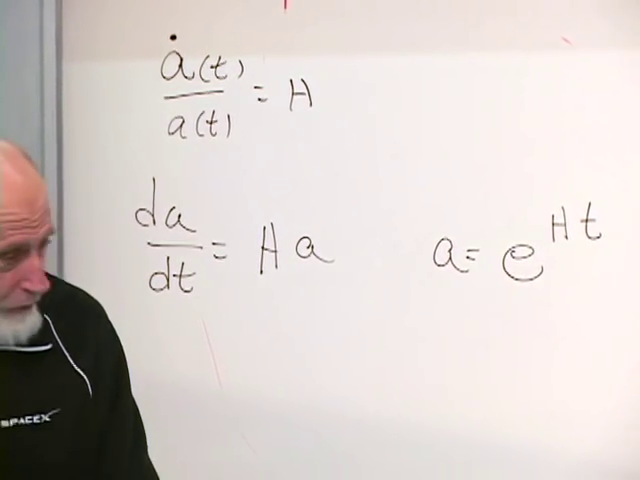
\includegraphics[width=0.70\textwidth]{lecture_07_figure_14.png}
\caption{黒板に書かれた一定の\(H\)に対する方程式とその指数関数解。}
\lectureframe{01:39:30.000}
\end{figure}

この指数的膨張を持つ時空はド・ジッター空間である。その一定のハッブルスケールは有限の固有距離に事象の地平面を生じる。この幾何はある意味でブラックホールの描像の補集合である。観測者は宇宙論的地平面の内側にとどまり、十分遠方の物体は後退して、観測者を捕まえる信号を決して送ることができない。ブラックホールの地平面は内部を外部の観測者から隠す。ド・ジッターの地平面は、観測者の到達可能なパッチの外部を隠す。普通の蒸発するブラックホールとは異なり、理想的なド・ジッター幾何はここでは持続するものとして扱われる。この比較はここで始まったばかりである。次の講義では、地平面、その熱力学、そしてそれが宇宙論にもたらす難題を展開する。
